\documentclass{standalone}
% 

% \pgfmathdeclarefunction{gauss}{2}{%
%   \pgfmathparse{1/(#2*sqrt(2*pi))*exp(-((x-#1)^2)/(2*#2^2))}%
% }
\usepackage{tkz-euclide}
\usetkzobj{all}
\renewcommand{\familydefault}{\sfdefault}
\usepackage{calc,tikz}
\usetikzlibrary{calc}
\usepackage{pgfplots}
\begin{document}
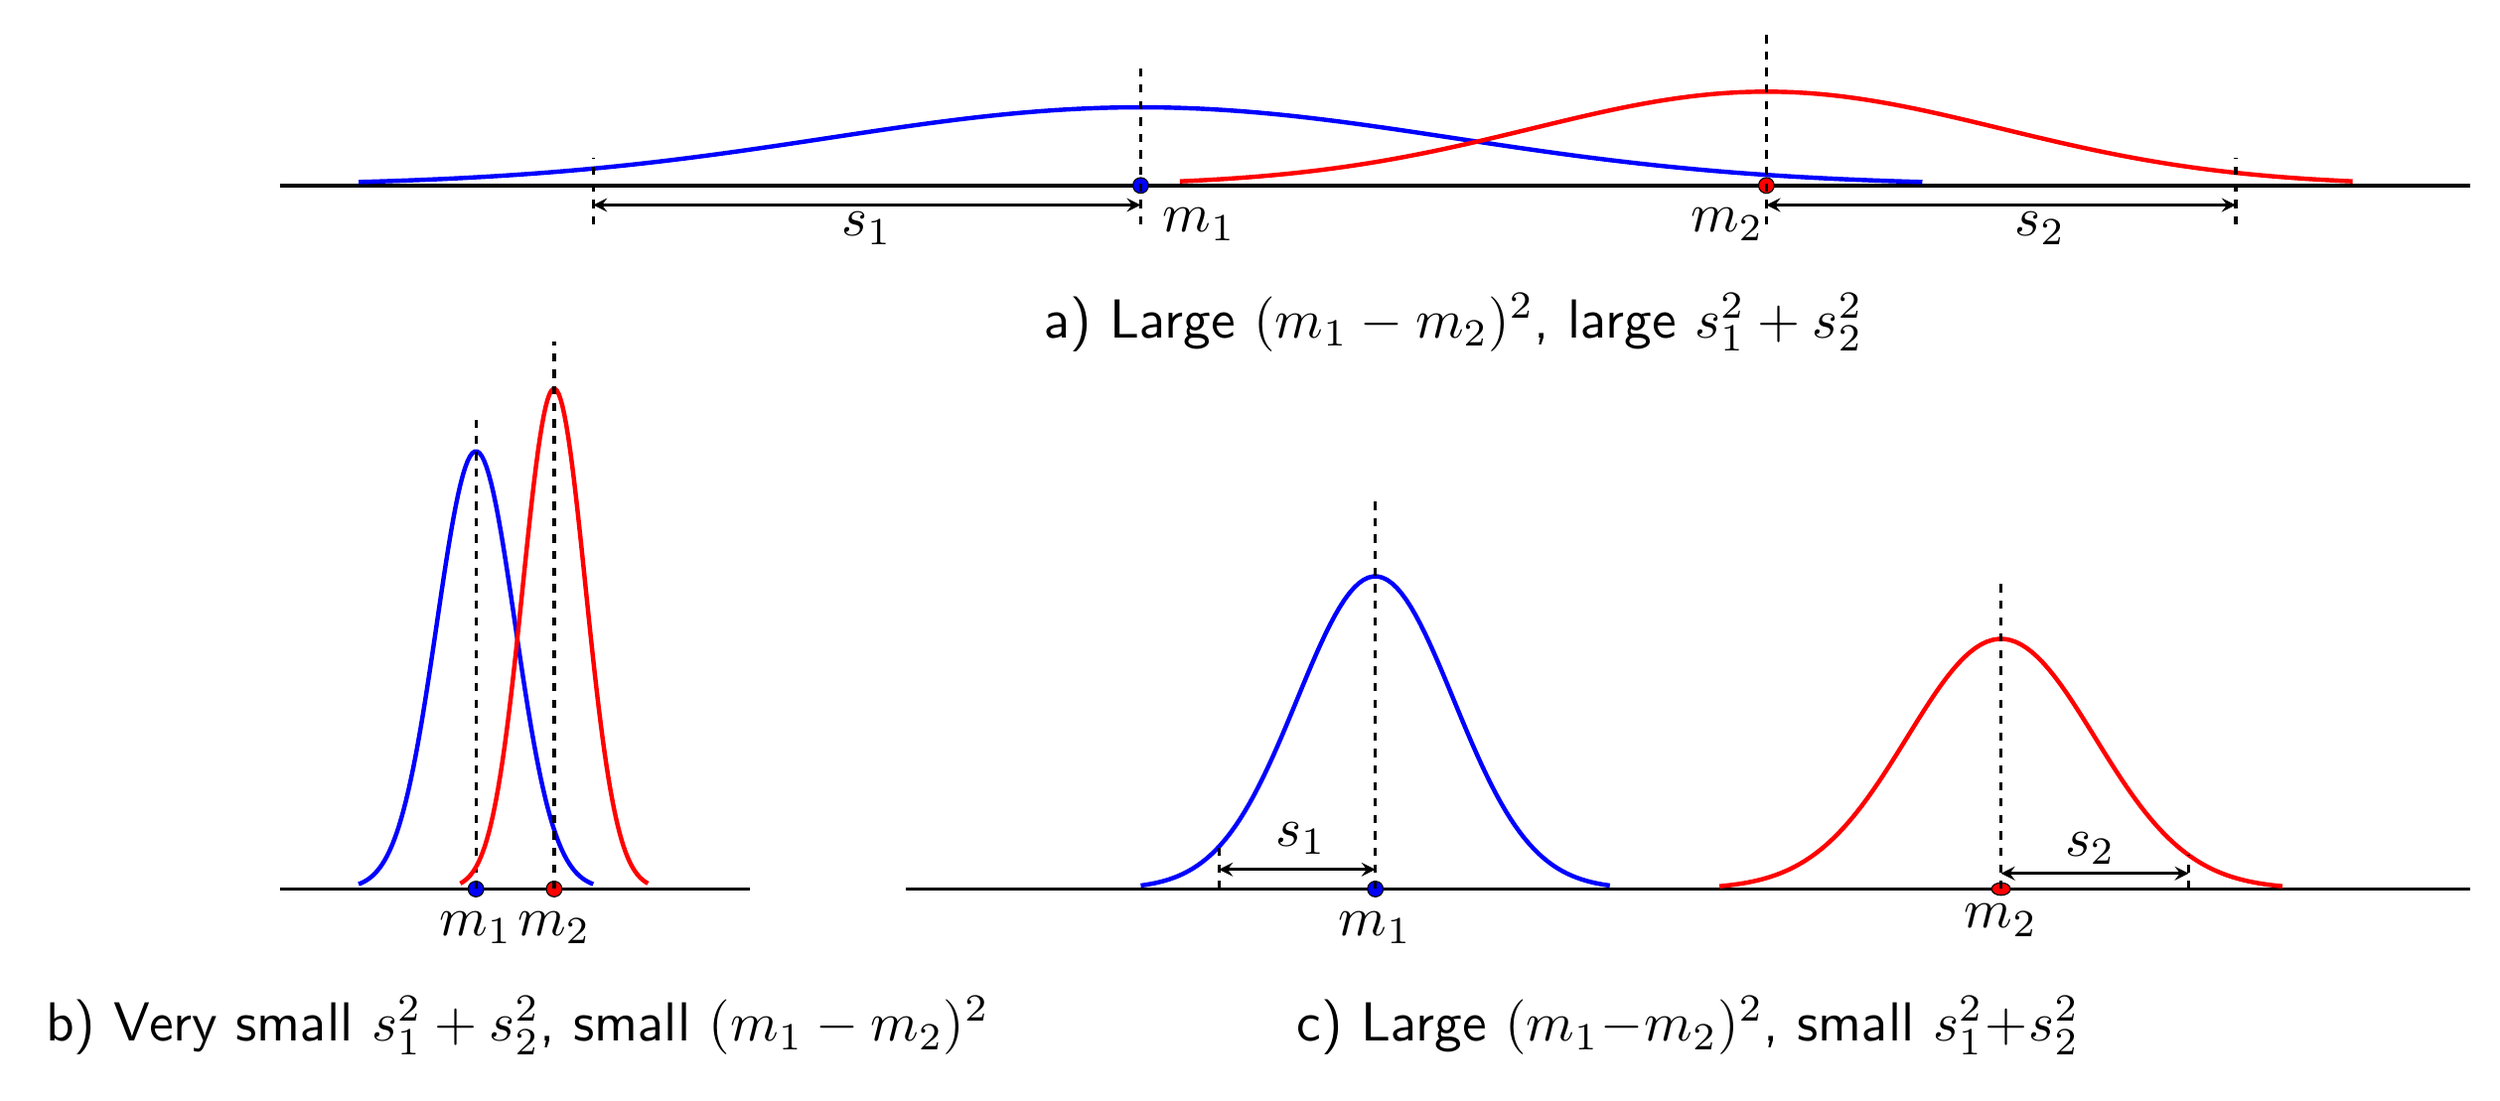
\begin{tikzpicture}[>=stealth]
    % \clip (-14.25, -1.4) rectangle (7.5, 7.2);
    \def\normaltwo{\x,{4*1/exp(((\x-0)^2)/2)}}


    \begin{scope}[xshift = 2 cm , yshift = 9cm]
        \draw [line width = .5mm] (-15, 0)  --  (13, 0);
        \begin{scope}[xshift = -4cm, xscale = 4, yscale = .25]
            \draw[color=blue,domain=-2.5:2.5, samples = 100, ultra thick] plot (\normaltwo) node[right] {};
        \end{scope}
            \draw [fill = blue] (-4, 0) circle (1mm);
            \node [scale = 2] at (-3.25, -.5) {$m_1$};
            \draw [dashed, very thick] (-4, -.5)  --  (-4, 1.5);
            \draw [dashed, very thick] (-11, -.5)  --  (-11, .35);
            \draw [<->, very thick] (-11, -.25)  --  (-4, -.25);
            \node [scale = 2] at (-7.5, -.55) {$s_1$};

        \begin{scope}[xshift = 4cm, xscale = 3, yscale = 0.3]
            \draw[color=red,domain=-2.5:2.5, samples = 100, ultra thick] plot (\normaltwo) node[right] {};
        \end{scope}
            \draw [fill = red] (4, 0) circle (1mm);
            \node [scale = 2] at (3.5, -.5) {$m_2$};
            \draw [dashed, very thick] (10, -.5)  --  (10, .35);
            \draw [dashed, very thick] (4, -.5)  --  (4, 2);
            \draw [<->, very thick] (4, -.25)  --  (10, -.25);
            \node [scale = 2] at (7.5, -.55) {$s_2$};
            \node [scale = 2] at (0, -1.75) {a) Large $(m_1 - m_2)^2$, large $s_1^2 + s_2^2$};

    \end{scope}


    \begin{scope}[xshift =-10 cm, yshift = 0cm]
        \draw [line width = .5mm] (-3, 0)  --  (3, 0);
        \begin{scope}[xshift = -.5cm, xscale = .5, yscale = 1.4]
            \draw[color=blue,domain=-3:3, samples = 100, ultra thick] plot (\normaltwo) node[right] {};
        \end{scope}
            \draw [fill = blue] (-.5, 0) circle (1mm);
            \node [scale = 2] at (-.5, -.5) {$m_1$};
            \draw [dashed, very thick] (-.5, 0)  --  (-0.5, 6);

        \begin{scope}[xshift = .5cm, xscale = .4, yscale = 1.6]
            \draw[color=red,domain=-3:3, samples = 100, ultra thick] plot (\normaltwo) node[right] {};
        \end{scope}
            \draw [fill = red] (.5, 0) circle (1mm);
            \node [scale = 2] at (.5, -.5) {$m_2$};
            % \draw [dashed, very thick] (1.5, 0)  --  (1.5, .45);
            \draw [dashed, very thick] (.5, 0)  --  (0.5, 7);

            \node [scale = 2, text width = 7cm] at (1, -1.75) {b) Very small $s_1^2 + s_2^2$, small $(m_1 - m_2)^2$};
    \end{scope}


    \begin{scope}[xshift = 5cm]
        \draw [line width = .5mm] (-10, 0)  --  (10, 0);
        \begin{scope}[xshift = -4cm]
            \draw[color=blue,domain=-3:3, samples = 100, ultra thick] plot (\normaltwo) node[right] {};
            \draw [fill = blue] (0, 0) circle (1mm);
            \node [scale = 2] at (0, -.5) {$m_1$};
            \node [scale = 2] at (-.95, .65) {$s_1$};
            \draw [dashed, very thick] (0, 0)  --  (0, 5);
            \draw [dashed, very thick] (-2, 0)  --  (-2, .55);
            \draw [<->, very thick] (-2, .25)  --  (0, .25);
        \end{scope}

        \begin{scope}[xshift = 4cm, xscale = 1.2, yscale = 0.8]
            \draw[color=red,domain=-3:3, samples = 100, ultra thick] plot (\normaltwo) node[right] {};
            \draw [fill = red] (0, 0) circle (1mm);
            \draw [dashed, very thick] (0, 0)  --  (0, 5);
            \node [scale = 2] at (0, -.5) {$m_2$};
            \draw [dashed, very thick] (2, 0)  --  (2, .55);
            \draw [<->, very thick] (2, .25)  --  (0, .25);
            \node [scale = 2] at (.95, .65) {$s_2$};
        \end{scope}
        \node [scale = 2, text width = 5cm] at (0, -1.75) {c) Large $(m_1 - m_2)^2$, small $s_1^2 + s_2^2$};

    \end{scope}
   
    

\end{tikzpicture}
\end{document}